% Igniting Coach — the default coaching agreement.
% Warm and plain-spoken by design, built on the ICF Code of Ethics (2025) and
% Core Competency 3, "Establishes and Maintains Agreements".
% Off-white on black, gold for the accents and the signatures; no frame, plenty of air.
% The top of page 1 carries a faint copy of the website's map (contract/map-svg.mjs).
%
% Build: contract/build.sh (lualatex, two runs) → public/contract/coaching-agreement.pdf
%
% Two pages. The signatures are laid out at fixed places on page 2: the contract page
% (src/pages/contract.astro) stamps the client's signature, name and date onto
% the last page at the same places. If you move anything in the SIGNATURES
% block below, move the matching numbers in src/lib/contract-sign.ts (SLOTS).

\documentclass[9pt]{extarticle}
\usepackage[a4paper,top=20mm,bottom=22mm,left=21mm,right=21mm,footskip=10mm]{geometry}
\usepackage{fontspec}
\usepackage{xcolor}
\usepackage{pagecolor}
\usepackage{tikz}
\usetikzlibrary{calc}
\usepackage{graphicx}
\usepackage{titlesec}
\usepackage{enumitem}
\usepackage{microtype}
\usepackage{fancyhdr}
\usepackage[most]{tcolorbox}
\usepackage{lastpage}
\usepackage{needspace}
\usepackage{multicol}
\usepackage[hidelinks]{hyperref}

\hypersetup{
  pdftitle={Our Coaching Agreement — Igniting Coach},
  pdfauthor={Ilya Malyarenko},
  pdfsubject={Coaching agreement, version 1.0},
}

% ---- colour: the page is black, the words off-white, the accents gold
\definecolor{ground}{HTML}{0B0B0C}
\definecolor{paper}{HTML}{ECE6DA}
\definecolor{soft}{HTML}{A8A296}
\definecolor{gold}{HTML}{C9A24E}
\definecolor{goldlight}{HTML}{E2C47C}
\definecolor{golddim}{HTML}{6E5A2C}
\pagecolor{ground}
\color{paper}

% ---- type: Inter Light to read (modern, open, easy on a dark page), Inter
% Display for headings and labels, GFS Didot for the title's flourish and the
% gold initials
\setmainfont{Inter-Light.otf}[
  ItalicFont=Inter-LightItalic.otf, BoldFont=Inter-Medium.otf, BoldItalicFont=Inter-MediumItalic.otf,
  Numbers={Proportional,Lining}, Ligatures=TeX]
\newfontfamily\display{InterDisplay-ExtraLight.otf}[ItalicFont=InterDisplay-ExtraLightItalic.otf, Ligatures=TeX]
\newfontfamily\head{InterDisplay-Light.otf}[Ligatures=TeX]
\newfontfamily\tracked{Inter-Medium.otf}[LetterSpace=22, Numbers=Lining]
\newfontfamily\didot{GFSDidot.otf}[ItalicFont=GFSDidotItalic.otf]
\linespread{1.14}
\setlength{\parindent}{0pt}
\setlength{\parskip}{4pt plus 1pt}
\frenchspacing

% ---- initials: a gold Didot capital, two lines deep
\usepackage{lettrine}
\setlength{\DefaultFindent}{1.2pt}
\setlength{\DefaultNindent}{0pt}
\renewcommand{\LettrineFontHook}{\didot\color{gold}}
\renewcommand{\LettrineTextFont}{\relax}
\newcommand{\initial}[2]{\lettrine[lines=2, loversize=.08, lraise=.02]{#1}{#2}}

% ---- a hairline: gold, fading out at both ends
\newcommand{\hairline}[1][\linewidth]{%
  \begin{tikzpicture}
    \shade[left color=ground, right color=gold, middle color=gold] (0,0) rectangle (#1/2,.35pt);
    \shade[left color=gold, right color=ground] (#1/2,0) rectangle (#1,.35pt);
  \end{tikzpicture}}

% ---- the running foot: the website and the page, small and spaced
\pagestyle{fancy}
\fancyhf{}
\renewcommand{\headrulewidth}{0pt}
\fancyfoot[L]{\tracked\fontsize{6}{8}\selectfont\color{gold}IGNITING.COACH}
\fancyfoot[R]{\tracked\fontsize{6}{8}\selectfont\color{soft}\thepage\,/\,\pageref{LastPage}}

% ---- sections: a small gold numeral, the heading in Inter Display
\renewcommand{\thesection}{\ifnum\value{section}<10 0\fi\arabic{section}}
\titleformat{\section}
  {\head\fontsize{12}{15}\selectfont\color{paper}}
  {\tracked\fontsize{6.5}{15}\selectfont\color{gold}\thesection\hspace{3mm}}
  {0pt}{}
\titlespacing*{\section}{0pt}{9pt}{3pt}

% ---- lists: a short gold dash
\newcommand{\golddash}{\tikz[baseline=-.6ex]\fill[gold] (0,-.2pt) rectangle (1.6mm,.2pt);}
\setlist[itemize]{label=\golddash, leftmargin=1.1em, labelsep=.5em, itemsep=1.4pt, topsep=2pt, parsep=0pt}

% ---- a quiet aside, in Inter Display italic with a gold rule beside it
\newtcolorbox{asidebox}{enhanced, frame hidden, colback=ground, boxrule=0pt, sharp corners,
  borderline west={.5pt}{0pt}{gold}, left=4mm, right=0mm, top=.5mm, bottom=.5mm,
  before skip=6pt, after skip=6pt}
\newcommand{\aside}[1]{\begin{asidebox}\display\itshape\fontsize{12.5}{16}\selectfont\color{goldlight}#1\end{asidebox}}

\setlength{\columnsep}{9mm}
\setlength{\multicolsep}{0pt}

\begin{document}

% =====================================================================
% PAGE 1 — the emblem and the title, a word from me, then the agreement
% =====================================================================
\thispagestyle{fancy}
% the website's map, faint, across the top of the page, fading out downwards
% (build/map.pdf, from contract/map-svg.mjs)
\begin{tikzpicture}[remember picture,overlay]
  \node[anchor=north west,inner sep=0] at (current page.north west) {\includegraphics[width=\paperwidth]{build/map.pdf}};
\end{tikzpicture}%
\begin{minipage}[t]{24mm}
  \vspace{0pt}\includegraphics[height=47mm]{build/torchbearer.pdf}
\end{minipage}\hspace{8mm}%
\begin{minipage}[t]{\dimexpr\linewidth-32mm}
  \vspace{1mm}
  {\tracked\fontsize{6.5}{8}\selectfont\color{gold}IGNITING COACH\hspace{1.4em}\color{soft}IGNITING.COACH\par}
  \vspace{4mm}
  {\display\fontsize{33}{35}\selectfont Our Coaching {\didot\itshape\color{goldlight}Agreement}\par}
  \vspace{3mm}
  {\fontsize{9.5}{13}\selectfont\color{soft}What we are agreeing to, in plain words, between {\color{paper}Ilya Malyarenko} of Igniting Coach and {\color{paper}you}.\par}
  \vspace{4.5mm}
  {\fontsize{9}{13.4}\selectfont\initial{W}{elcome.} I'm glad you're here. Choosing to work with a coach takes a little courage. These two pages describe how we'll work together, so that neither of us has to guess: the conversation we'd have over coffee, kept on paper. They follow the Code of Ethics and the core competencies of the International Coaching Federation (ICF). If anything doesn't sit right with you, tell me before you sign, and we'll talk it through.\par}
  \vspace{2mm}
  {\didot\itshape\fontsize{15}{17}\selectfont\color{gold}Ilya\par}
\end{minipage}

\vspace{6mm}
\hairline
\vspace{2mm}

\begin{multicols}{2}
\raggedcolumns

\section{What coaching is, and what it isn't}
\initial{C}{oaching} is a partnership of equals. I ask questions, listen closely and reflect back what I notice; you do the thinking, choosing and acting. You are the expert on your own life.

Coaching is not therapy, counselling, or medical, legal or financial advice. In our sessions I am your coach and nothing else. If something you bring would be better served by another professional, I'll say so openly and help you find the right person (the IACP register at \href{https://iacp.ie/therapists}{\color{goldlight}iacp.ie} is a good start). I never receive anything for referring you to anyone.

\section{How we'll work together}
\begin{itemize}
  \item A free \emph{chemistry call} of about thirty minutes first, to see whether we're a good fit. No obligation, either way.
  \item Usually four to eight sessions of about an hour, two to eight weeks apart. The time between sessions is where the thinking lands.
  \item In person or online by video, in English or Russian.
  \item We'll agree what you want from coaching as a whole, and at each session what you'd like to leave with. Either can change whenever you need it to.
  \item Around the fifth session we'll take stock. If things aren't moving, we'll say so honestly and decide together what next.
\end{itemize}

\section{Fees}
\initial{T}{he chemistry} call is free. Before your first paid session I'll confirm by email the fee for each session and how to pay. That email becomes part of this agreement. A fee only ever changes for sessions not yet booked, and only once you've agreed.

\section{When life gets in the way}
\initial{L}{et me} know at least 48 hours before if you need to move a session, and we'll simply find another time. With less notice the session normally counts as held, but I'm human about real emergencies. If I have to cancel, you'll get a new time straight away and never pay for it.

\aside{Coaching works best when you feel free to say the true thing, even when it surprises you.}

\section{What stays between us}
Everything you share is confidential, and I won't tell anyone you're my client without your permission. Only a few situations could make me share something, and wherever I can I'll talk with you first:
\begin{itemize}
  \item a serious risk of harm to you or to someone else;
  \item something Irish law requires me to report, such as a concern for a child's safety;
  \item an order from a court or another lawful authority.
\end{itemize}
I may discuss my work with a coaching supervisor, never with your name or anything that identifies you. Sessions are not recorded unless we both agree beforehand.

\end{multicols}

\newpage
% =====================================================================
% PAGE 2 — the rest, then our signatures at the foot
% =====================================================================
\begin{multicols}{2}
\raggedcolumns

\section{If someone else is paying}
\initial{S}{hould an} employer or another organisation pay, the three of us will agree in writing, before we start, what they will hear. Unless you agree otherwise, that's only whether sessions took place, and the invoices.

\section{Your information}
\initial{Y}{our information} is in my care, as Ilya Malyarenko, under data protection law (the GDPR).
\begin{itemize}
  \item \emph{What I keep:} your contact details, this agreement, invoices, and short session notes.
  \item \emph{Why:} to coach you and run my practice, on the basis of this agreement, and of your explicit consent for anything sensitive you share, such as your health.
  \item \emph{How:} on encrypted devices and secure services. Your words never go into artificial-intelligence tools without your explicit permission.
  \item \emph{How long:} session notes until a year after our last session; the agreement and invoices for six years, as Irish tax law requires.
  \item \emph{Your rights:} to see, correct or delete it, limit or object to its use, take a copy, or withdraw consent at any time. Just ask. You can also complain to the Data Protection Commission (\href{https://www.dataprotection.ie}{\color{goldlight}dataprotection.ie}).
\end{itemize}

\section{What you can expect from me}
\begin{itemize}
  \item My full attention, careful preparation, and honesty, including if I think coaching isn't helping.
  \item Work that follows the ICF Code of Ethics, with clear boundaries; our relationship stays a professional one.
  \item Openness about any conflict of interest, raised with you as soon as I see it.
  \item Care with the influence a coach can hold: I'll keep checking that our work serves you.
  \item My qualification, stated plainly: a Diploma in Personal \& Business Coaching from the Irish Lifecoach Institute (ICF Level~1).
\end{itemize}

\section{What I'll ask of you}
\begin{itemize}
  \item Come as you are, and be honest, including when something isn't working.
  \item Your choices, actions and results are yours. That's where the power of coaching lies.
  \item Tell me about anything coaching should fit around, such as therapy or medical treatment.
  \item Give the time between sessions a little of your attention.
\end{itemize}

\section{Ending well}
\initial{E}{ither} of us can end our work at any time, for any reason, simply by telling the other; an email is enough. There's no penalty, and sessions paid for but not held are refunded. If you like, we'll close with a last conversation about what has changed.

\section{A few last things}
\begin{itemize}
  \item You confirm that you are 18 or over.
  \item What you take from coaching depends on you, so I can't promise particular results, and your decisions are your own. Your rights as a consumer under Irish law are unaffected.
  \item This agreement and the email confirming your fee are everything we've agreed; changes are made in writing, and an email is fine. Irish law applies.
  \item We sign electronically. That's as binding as ink, and each of us keeps a copy.
\end{itemize}

\end{multicols}

% =====================================================================
% SIGNATURES — at fixed places on page 2 (see SLOTS in src/lib/contract-sign.ts).
% The words above must end higher than 110 mm from the foot of the page.
% =====================================================================
\begin{tikzpicture}[remember picture,overlay,x=1mm,y=1mm]
  \coordinate (o) at (current page.south west);
  \node[anchor=south west,inner sep=0] at ($(o)+(21,104.5)$) {\hairline[168mm]};
  \node[anchor=base west,inner sep=0] at ($(o)+(21,94)$) {\display\fontsize{17}{19}\selectfont\color{paper}Our {\didot\itshape\color{goldlight}signatures}};
  % two columns: the coach (x 21–97 mm), the client (x 113–189 mm); two lines
  % each: the signature, with the party and their name beneath it, and the date
  \foreach \x/\who in {21/COACH, 113/CLIENT} {
    % the signature: a line at 62 mm, room above it to 86 mm
    \draw[gold,line width=.4pt] ($(o)+(\x,62)$) -- ++(76,0);
    \node[anchor=base west,inner sep=0] at ($(o)+(\x,57)$) {\tracked\fontsize{5.5}{7}\selectfont\color{gold}\who};
    % the date: a line at 42 mm
    \draw[golddim,line width=.3pt] ($(o)+(\x,42)$) -- ++(76,0);
    \node[anchor=base west,inner sep=0] at ($(o)+(\x,37.5)$) {\tracked\fontsize{5}{7}\selectfont\color{soft}DATE};
  }
  % the coach's side: the signature in gold, the name once (it is legible as it is)
  \node[anchor=base west,inner sep=0] at ($(o)+(23,66)$) {\didot\itshape\fontsize{24}{26}\selectfont\color{gold}Ilya Malyarenko};
  \node[anchor=base,inner sep=0] at ($(o)+(105,27)$)
    {\fontsize{7}{9}\selectfont\color{soft}Signed electronically at igniting.coach; the date is added for both of us the moment you sign. Thank you for trusting me with this part of your life.};
\end{tikzpicture}

\end{document}
